% Created by tikzDevice version 0.6.2-92-0ad2792 on 2013-02-14 17:55:07
% !TEX encoding = UTF-8 Unicode
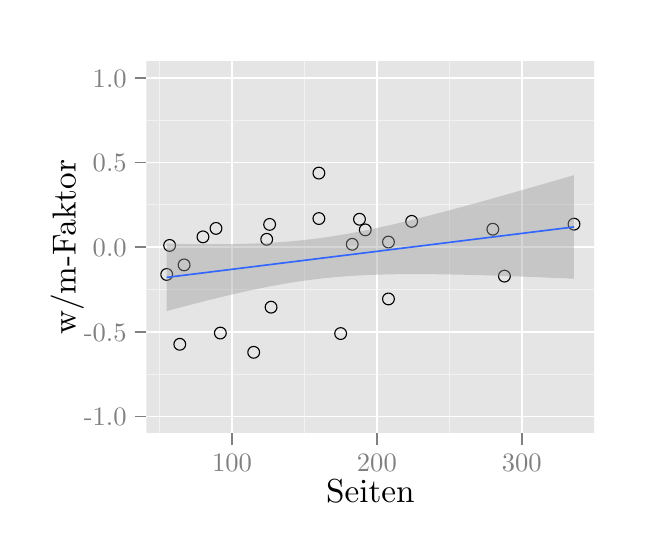
\begin{tikzpicture}[x=1pt,y=1pt]
\definecolor[named]{fillColor}{rgb}{1.00,1.00,1.00}
\path[use as bounding box,fill=fillColor,fill opacity=0.00] (0,0) rectangle (216.81,180.67);
\begin{scope}
\path[clip] (  0.00,  0.00) rectangle (216.81,180.67);
\definecolor[named]{drawColor}{rgb}{1.00,1.00,1.00}
\definecolor[named]{fillColor}{rgb}{1.00,1.00,1.00}

\path[draw=drawColor,line width= 0.6pt,line join=round,line cap=round,fill=fillColor] (  0.00,  0.00) rectangle (216.81,180.68);
\end{scope}
\begin{scope}
\path[clip] ( 42.89, 34.03) rectangle (204.77,168.63);
\definecolor[named]{fillColor}{rgb}{0.90,0.90,0.90}

\path[fill=fillColor] ( 42.89, 34.03) rectangle (204.77,168.63);
\definecolor[named]{drawColor}{rgb}{0.95,0.95,0.95}

\path[draw=drawColor,line width= 0.3pt,line join=round] ( 42.89, 55.45) --
	(204.77, 55.45);

\path[draw=drawColor,line width= 0.3pt,line join=round] ( 42.89, 86.04) --
	(204.77, 86.04);

\path[draw=drawColor,line width= 0.3pt,line join=round] ( 42.89,116.63) --
	(204.77,116.63);

\path[draw=drawColor,line width= 0.3pt,line join=round] ( 42.89,147.22) --
	(204.77,147.22);

\path[draw=drawColor,line width= 0.3pt,line join=round] ( 47.63, 34.03) --
	( 47.63,168.63);

\path[draw=drawColor,line width= 0.3pt,line join=round] (100.00, 34.03) --
	(100.00,168.63);

\path[draw=drawColor,line width= 0.3pt,line join=round] (152.37, 34.03) --
	(152.37,168.63);

\path[draw=drawColor,line width= 0.3pt,line join=round] (204.74, 34.03) --
	(204.74,168.63);
\definecolor[named]{drawColor}{rgb}{1.00,1.00,1.00}

\path[draw=drawColor,line width= 0.6pt,line join=round] ( 42.89, 40.15) --
	(204.77, 40.15);

\path[draw=drawColor,line width= 0.6pt,line join=round] ( 42.89, 70.74) --
	(204.77, 70.74);

\path[draw=drawColor,line width= 0.6pt,line join=round] ( 42.89,101.33) --
	(204.77,101.33);

\path[draw=drawColor,line width= 0.6pt,line join=round] ( 42.89,131.92) --
	(204.77,131.92);

\path[draw=drawColor,line width= 0.6pt,line join=round] ( 42.89,162.51) --
	(204.77,162.51);

\path[draw=drawColor,line width= 0.6pt,line join=round] ( 73.81, 34.03) --
	( 73.81,168.63);

\path[draw=drawColor,line width= 0.6pt,line join=round] (126.18, 34.03) --
	(126.18,168.63);

\path[draw=drawColor,line width= 0.6pt,line join=round] (178.55, 34.03) --
	(178.55,168.63);
\definecolor[named]{drawColor}{rgb}{0.00,0.00,0.00}

\path[draw=drawColor,line width= 0.4pt,line join=round,line cap=round] (105.23,128.12) circle (  2.13);

\path[draw=drawColor,line width= 0.4pt,line join=round,line cap=round] (105.23,111.70) circle (  2.13);

\path[draw=drawColor,line width= 0.4pt,line join=round,line cap=round] (119.90,111.44) circle (  2.13);

\path[draw=drawColor,line width= 0.4pt,line join=round,line cap=round] (138.75,110.68) circle (  2.13);

\path[draw=drawColor,line width= 0.4pt,line join=round,line cap=round] (197.41,109.67) circle (  2.13);

\path[draw=drawColor,line width= 0.4pt,line join=round,line cap=round] ( 87.43,109.58) circle (  2.13);

\path[draw=drawColor,line width= 0.4pt,line join=round,line cap=round] ( 68.05,108.13) circle (  2.13);

\path[draw=drawColor,line width= 0.4pt,line join=round,line cap=round] (168.08,107.84) circle (  2.13);

\path[draw=drawColor,line width= 0.4pt,line join=round,line cap=round] (121.99,107.60) circle (  2.13);

\path[draw=drawColor,line width= 0.4pt,line join=round,line cap=round] ( 63.34,105.08) circle (  2.13);

\path[draw=drawColor,line width= 0.4pt,line join=round,line cap=round] ( 86.38,104.19) circle (  2.13);

\path[draw=drawColor,line width= 0.4pt,line join=round,line cap=round] (130.37,103.21) circle (  2.13);

\path[draw=drawColor,line width= 0.4pt,line join=round,line cap=round] (117.28,102.39) circle (  2.13);

\path[draw=drawColor,line width= 0.4pt,line join=round,line cap=round] ( 51.29,101.98) circle (  2.13);

\path[draw=drawColor,line width= 0.4pt,line join=round,line cap=round] ( 56.53, 94.95) circle (  2.13);

\path[draw=drawColor,line width= 0.4pt,line join=round,line cap=round] ( 50.24, 91.49) circle (  2.13);

\path[draw=drawColor,line width= 0.4pt,line join=round,line cap=round] (172.27, 90.89) circle (  2.13);

\path[draw=drawColor,line width= 0.4pt,line join=round,line cap=round] (130.37, 82.64) circle (  2.13);

\path[draw=drawColor,line width= 0.4pt,line join=round,line cap=round] ( 87.95, 79.67) circle (  2.13);

\path[draw=drawColor,line width= 0.4pt,line join=round,line cap=round] ( 69.62, 70.32) circle (  2.13);

\path[draw=drawColor,line width= 0.4pt,line join=round,line cap=round] (113.09, 70.14) circle (  2.13);

\path[draw=drawColor,line width= 0.4pt,line join=round,line cap=round] ( 54.96, 66.26) circle (  2.13);

\path[draw=drawColor,line width= 0.4pt,line join=round,line cap=round] ( 81.67, 63.36) circle (  2.13);
\definecolor[named]{fillColor}{rgb}{0.60,0.60,0.60}

\path[fill=fillColor,fill opacity=0.40] ( 50.24,102.62) --
	( 52.11,102.58) --
	( 53.97,102.54) --
	( 55.83,102.51) --
	( 57.70,102.48) --
	( 59.56,102.45) --
	( 61.42,102.43) --
	( 63.28,102.42) --
	( 65.15,102.41) --
	( 67.01,102.41) --
	( 68.87,102.41) --
	( 70.73,102.43) --
	( 72.60,102.44) --
	( 74.46,102.47) --
	( 76.32,102.51) --
	( 78.19,102.55) --
	( 80.05,102.60) --
	( 81.91,102.67) --
	( 83.77,102.74) --
	( 85.64,102.83) --
	( 87.50,102.93) --
	( 89.36,103.04) --
	( 91.23,103.16) --
	( 93.09,103.30) --
	( 94.95,103.45) --
	( 96.81,103.62) --
	( 98.68,103.81) --
	(100.54,104.00) --
	(102.40,104.22) --
	(104.27,104.45) --
	(106.13,104.70) --
	(107.99,104.96) --
	(109.85,105.24) --
	(111.72,105.53) --
	(113.58,105.84) --
	(115.44,106.16) --
	(117.31,106.50) --
	(119.17,106.85) --
	(121.03,107.21) --
	(122.89,107.58) --
	(124.76,107.97) --
	(126.62,108.37) --
	(128.48,108.77) --
	(130.35,109.19) --
	(132.21,109.62) --
	(134.07,110.05) --
	(135.93,110.49) --
	(137.80,110.94) --
	(139.66,111.40) --
	(141.52,111.87) --
	(143.39,112.33) --
	(145.25,112.81) --
	(147.11,113.29) --
	(148.97,113.78) --
	(150.84,114.27) --
	(152.70,114.76) --
	(154.56,115.26) --
	(156.42,115.76) --
	(158.29,116.26) --
	(160.15,116.77) --
	(162.01,117.28) --
	(163.88,117.80) --
	(165.74,118.32) --
	(167.60,118.83) --
	(169.46,119.36) --
	(171.33,119.88) --
	(173.19,120.41) --
	(175.05,120.93) --
	(176.92,121.46) --
	(178.78,122.00) --
	(180.64,122.53) --
	(182.50,123.06) --
	(184.37,123.60) --
	(186.23,124.14) --
	(188.09,124.68) --
	(189.96,125.22) --
	(191.82,125.76) --
	(193.68,126.30) --
	(195.54,126.84) --
	(197.41,127.39) --
	(197.41, 89.94) --
	(195.54, 90.02) --
	(193.68, 90.10) --
	(191.82, 90.18) --
	(189.96, 90.26) --
	(188.09, 90.34) --
	(186.23, 90.42) --
	(184.37, 90.50) --
	(182.50, 90.57) --
	(180.64, 90.64) --
	(178.78, 90.72) --
	(176.92, 90.79) --
	(175.05, 90.85) --
	(173.19, 90.92) --
	(171.33, 90.98) --
	(169.46, 91.05) --
	(167.60, 91.11) --
	(165.74, 91.17) --
	(163.88, 91.22) --
	(162.01, 91.27) --
	(160.15, 91.32) --
	(158.29, 91.37) --
	(156.42, 91.41) --
	(154.56, 91.45) --
	(152.70, 91.49) --
	(150.84, 91.52) --
	(148.97, 91.55) --
	(147.11, 91.58) --
	(145.25, 91.59) --
	(143.39, 91.61) --
	(141.52, 91.62) --
	(139.66, 91.62) --
	(137.80, 91.61) --
	(135.93, 91.60) --
	(134.07, 91.58) --
	(132.21, 91.56) --
	(130.35, 91.52) --
	(128.48, 91.48) --
	(126.62, 91.42) --
	(124.76, 91.36) --
	(122.89, 91.28) --
	(121.03, 91.20) --
	(119.17, 91.10) --
	(117.31, 90.99) --
	(115.44, 90.86) --
	(113.58, 90.72) --
	(111.72, 90.57) --
	(109.85, 90.40) --
	(107.99, 90.22) --
	(106.13, 90.02) --
	(104.27, 89.80) --
	(102.40, 89.57) --
	(100.54, 89.32) --
	( 98.68, 89.06) --
	( 96.81, 88.78) --
	( 94.95, 88.49) --
	( 93.09, 88.18) --
	( 91.23, 87.86) --
	( 89.36, 87.52) --
	( 87.50, 87.17) --
	( 85.64, 86.81) --
	( 83.77, 86.43) --
	( 81.91, 86.05) --
	( 80.05, 85.65) --
	( 78.19, 85.24) --
	( 76.32, 84.82) --
	( 74.46, 84.40) --
	( 72.60, 83.96) --
	( 70.73, 83.52) --
	( 68.87, 83.07) --
	( 67.01, 82.61) --
	( 65.15, 82.15) --
	( 63.28, 81.68) --
	( 61.42, 81.20) --
	( 59.56, 80.72) --
	( 57.70, 80.24) --
	( 55.83, 79.75) --
	( 53.97, 79.25) --
	( 52.11, 78.75) --
	( 50.24, 78.25) --
	cycle;
\definecolor[named]{drawColor}{rgb}{0.20,0.40,1.00}

\path[draw=drawColor,line width= 0.6pt,line join=round] ( 50.24, 90.43) --
	( 52.11, 90.66) --
	( 53.97, 90.90) --
	( 55.83, 91.13) --
	( 57.70, 91.36) --
	( 59.56, 91.59) --
	( 61.42, 91.82) --
	( 63.28, 92.05) --
	( 65.15, 92.28) --
	( 67.01, 92.51) --
	( 68.87, 92.74) --
	( 70.73, 92.97) --
	( 72.60, 93.20) --
	( 74.46, 93.43) --
	( 76.32, 93.66) --
	( 78.19, 93.90) --
	( 80.05, 94.13) --
	( 81.91, 94.36) --
	( 83.77, 94.59) --
	( 85.64, 94.82) --
	( 87.50, 95.05) --
	( 89.36, 95.28) --
	( 91.23, 95.51) --
	( 93.09, 95.74) --
	( 94.95, 95.97) --
	( 96.81, 96.20) --
	( 98.68, 96.43) --
	(100.54, 96.66) --
	(102.40, 96.89) --
	(104.27, 97.13) --
	(106.13, 97.36) --
	(107.99, 97.59) --
	(109.85, 97.82) --
	(111.72, 98.05) --
	(113.58, 98.28) --
	(115.44, 98.51) --
	(117.31, 98.74) --
	(119.17, 98.97) --
	(121.03, 99.20) --
	(122.89, 99.43) --
	(124.76, 99.66) --
	(126.62, 99.89) --
	(128.48,100.13) --
	(130.35,100.36) --
	(132.21,100.59) --
	(134.07,100.82) --
	(135.93,101.05) --
	(137.80,101.28) --
	(139.66,101.51) --
	(141.52,101.74) --
	(143.39,101.97) --
	(145.25,102.20) --
	(147.11,102.43) --
	(148.97,102.66) --
	(150.84,102.89) --
	(152.70,103.12) --
	(154.56,103.36) --
	(156.42,103.59) --
	(158.29,103.82) --
	(160.15,104.05) --
	(162.01,104.28) --
	(163.88,104.51) --
	(165.74,104.74) --
	(167.60,104.97) --
	(169.46,105.20) --
	(171.33,105.43) --
	(173.19,105.66) --
	(175.05,105.89) --
	(176.92,106.12) --
	(178.78,106.36) --
	(180.64,106.59) --
	(182.50,106.82) --
	(184.37,107.05) --
	(186.23,107.28) --
	(188.09,107.51) --
	(189.96,107.74) --
	(191.82,107.97) --
	(193.68,108.20) --
	(195.54,108.43) --
	(197.41,108.66);
\end{scope}
\begin{scope}
\path[clip] (  0.00,  0.00) rectangle (216.81,180.67);
\definecolor[named]{drawColor}{rgb}{0.50,0.50,0.50}

\node[text=drawColor,anchor=base east,inner sep=0pt, outer sep=0pt, scale=  0.96] at ( 35.77, 36.85) {-1.0};

\node[text=drawColor,anchor=base east,inner sep=0pt, outer sep=0pt, scale=  0.96] at ( 35.77, 67.44) {-0.5};

\node[text=drawColor,anchor=base east,inner sep=0pt, outer sep=0pt, scale=  0.96] at ( 35.77, 98.03) {0.0};

\node[text=drawColor,anchor=base east,inner sep=0pt, outer sep=0pt, scale=  0.96] at ( 35.77,128.62) {0.5};

\node[text=drawColor,anchor=base east,inner sep=0pt, outer sep=0pt, scale=  0.96] at ( 35.77,159.21) {1.0};
\end{scope}
\begin{scope}
\path[clip] (  0.00,  0.00) rectangle (216.81,180.67);
\definecolor[named]{drawColor}{rgb}{0.50,0.50,0.50}

\path[draw=drawColor,line width= 0.6pt,line join=round] ( 38.62, 40.15) --
	( 42.89, 40.15);

\path[draw=drawColor,line width= 0.6pt,line join=round] ( 38.62, 70.74) --
	( 42.89, 70.74);

\path[draw=drawColor,line width= 0.6pt,line join=round] ( 38.62,101.33) --
	( 42.89,101.33);

\path[draw=drawColor,line width= 0.6pt,line join=round] ( 38.62,131.92) --
	( 42.89,131.92);

\path[draw=drawColor,line width= 0.6pt,line join=round] ( 38.62,162.51) --
	( 42.89,162.51);
\end{scope}
\begin{scope}
\path[clip] (  0.00,  0.00) rectangle (216.81,180.67);
\definecolor[named]{drawColor}{rgb}{0.50,0.50,0.50}

\path[draw=drawColor,line width= 0.6pt,line join=round] ( 73.81, 29.77) --
	( 73.81, 34.03);

\path[draw=drawColor,line width= 0.6pt,line join=round] (126.18, 29.77) --
	(126.18, 34.03);

\path[draw=drawColor,line width= 0.6pt,line join=round] (178.55, 29.77) --
	(178.55, 34.03);
\end{scope}
\begin{scope}
\path[clip] (  0.00,  0.00) rectangle (216.81,180.67);
\definecolor[named]{drawColor}{rgb}{0.50,0.50,0.50}

\node[text=drawColor,anchor=base,inner sep=0pt, outer sep=0pt, scale=  0.96] at ( 73.81, 20.31) {100};

\node[text=drawColor,anchor=base,inner sep=0pt, outer sep=0pt, scale=  0.96] at (126.18, 20.31) {200};

\node[text=drawColor,anchor=base,inner sep=0pt, outer sep=0pt, scale=  0.96] at (178.55, 20.31) {300};
\end{scope}
\begin{scope}
\path[clip] (  0.00,  0.00) rectangle (216.81,180.67);
\definecolor[named]{drawColor}{rgb}{0.00,0.00,0.00}

\node[text=drawColor,anchor=base,inner sep=0pt, outer sep=0pt, scale=  1.20] at (123.83,  9.03) {Seiten};
\end{scope}
\begin{scope}
\path[clip] (  0.00,  0.00) rectangle (216.81,180.67);
\definecolor[named]{drawColor}{rgb}{0.00,0.00,0.00}

\node[text=drawColor,rotate= 90.00,anchor=base,inner sep=0pt, outer sep=0pt, scale=  1.20] at ( 17.30,101.33) {w/m-Faktor};
\end{scope}
\end{tikzpicture}
